\subsection{M.PD.5 - Completezza descrittiva}
 \begin{figure}[H]
    \centering
    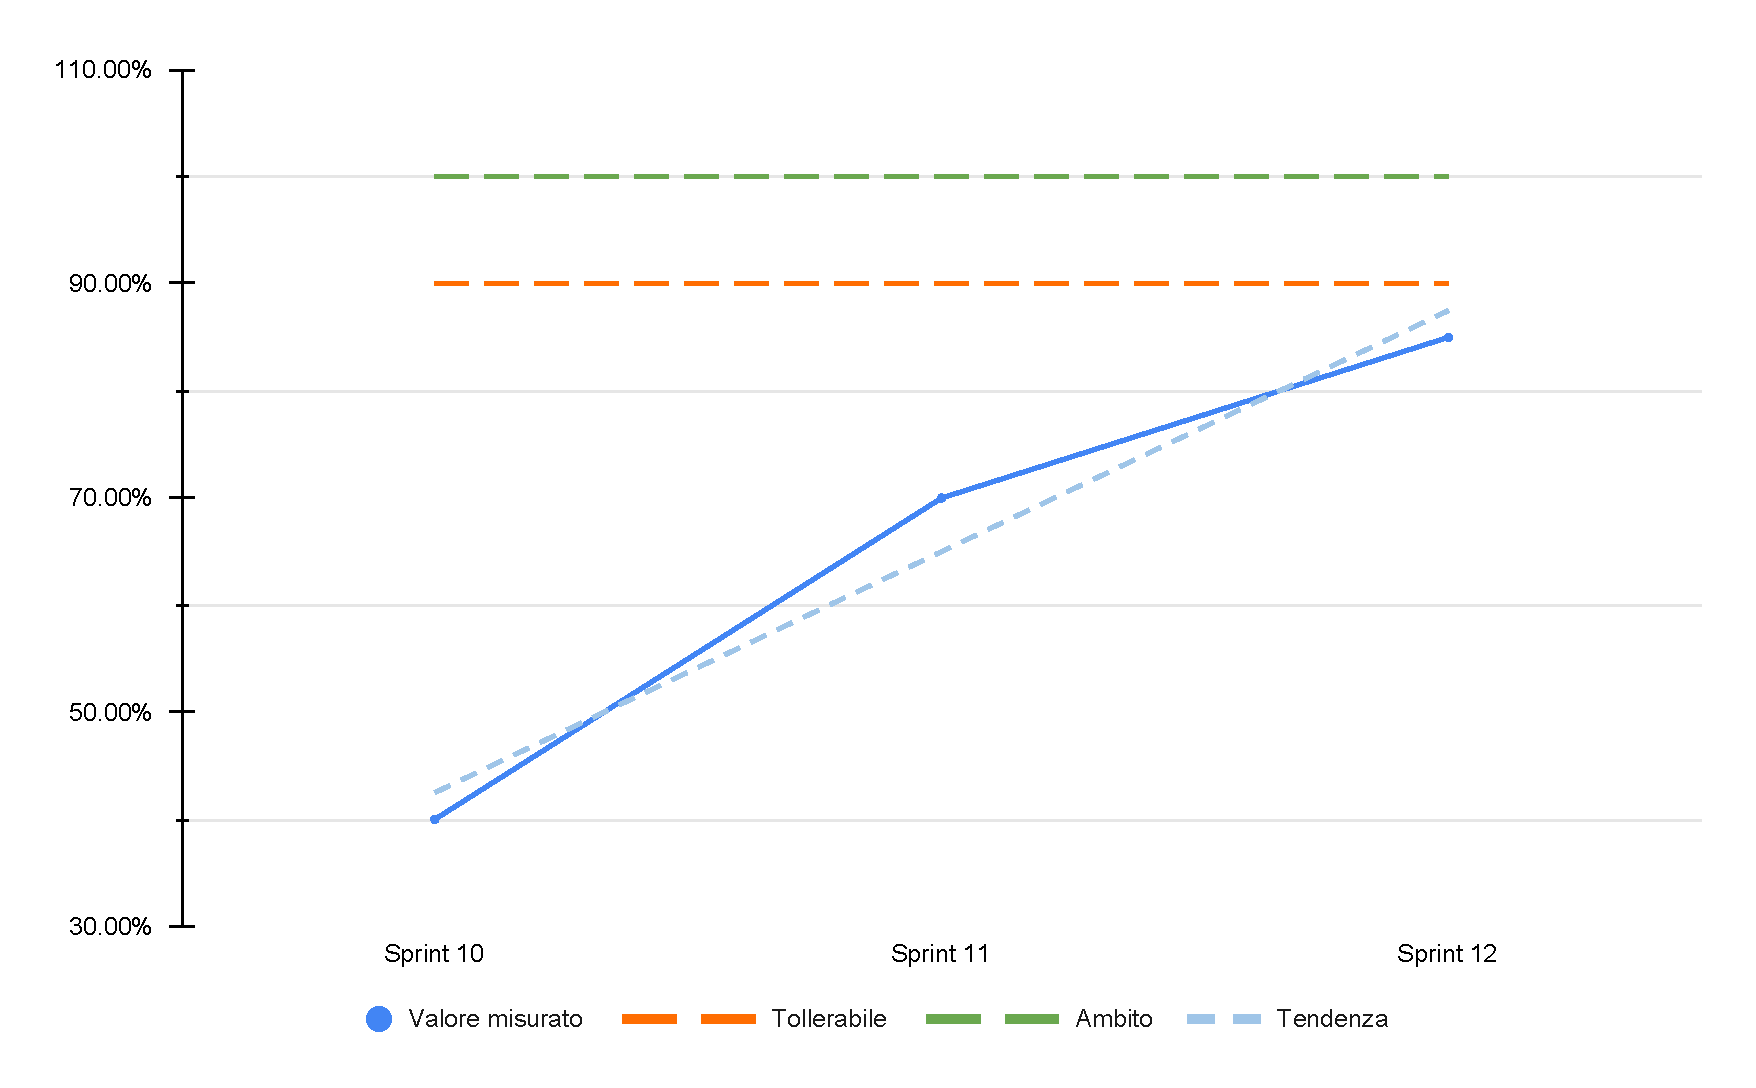
\includegraphics[width=\textwidth]{assets/completezza_descrittiva.pdf}
    \caption{M.PD.5 - Completezza descrittiva}
\end{figure}

\par Nei primi due sprint della \glossario{PB}, le funzioni sviluppate non sono state documentate adeguatamente, poiché il team era focalizzato sulle attività di progettazione, codifica e configurazione dei test. Di conseguenza, il valore misurato è rimasto al di sotto della soglia accettabile. A partire dallo \glossario{sprint} 12, il gruppo ha esteso la completezza descrittiva integrando commenti nel codice e ampliando il documento di \ST. Questo ha permesso al team di ottimizzare le fasi di testing e manutenzione del codice.